\documentclass{beamer}
\mode<presentation>
\usetheme{Madrid}
\usecolortheme{crane}

\usepackage{tikz}
\usepackage{epic}
\usepackage{tikz-qtree}
\usepackage{linguex}
\usepackage[normalem]{ulem}
\usepackage{tikz-dependency}
\usepackage{colortbl}
\usepackage{xcolor}
\definecolor{darkgreen}{rgb}{0,0.3,0}
\definecolor{darkblue}{rgb}{.05,.05,.30}
\definecolor{lightgrey}{rgb}{0.65,0.65,0.65}
\usepackage{tikzsymbols}
\usepackage{amsmath}
\usepackage{multirow}

\newcommand{\norm}[1]{\left\lVert#1\right\rVert}
\newcommand{\remph}[1]{\textbf{\color{red} #1}}


\title[LT2222 lecture 3]{LT2222 Machine learning for NLP: intro, Winter 2021}
\subtitle{Lecture 3: Vector spaces, word and document; Maximum entropy}
\author[Sayeed]{Asad Sayeed\\{\small with content from Jon Dehdari}}
\institute[Gothenburg]{University of Gothenburg}
\date{}

\setbeamertemplate{navigation symbols}{}

\newcommand{\placard}[1]{
  \begin{frame}
    \begin{center}
      \huge
      \textbf{#1}
    \end{center}
  \end{frame}
}

\newcommand{\pagestep}[2]{
  \begin{frame}[t]
    \begin{minipage}[t][0.26\textheight][t]{\textwidth}
      \begin{center}
        \huge
        \textbf{#1}
      \end{center}
    \end{minipage}
    
    \begin{minipage}[t][0.7\textheight][c]{\textwidth}
      \begin{center}
        \includegraphics[height=0.83\textheight]{#2}
      \end{center}
    \end{minipage}
  \end{frame}
}

\newcommand{\pagestepalt}[2]{
  \begin{frame}[t]
    \begin{minipage}[t][0.26\textheight][t]{\textwidth}
      \begin{center}
        \huge
        \textbf{#1}
      \end{center}
    \end{minipage}
    
    \begin{minipage}[t][0.7\textheight][c]{\textwidth}
      #2
    \end{minipage}
  \end{frame}
}

%% \newcommand{\pagestepaltfragile}[2]{
%%   \begin{frame}[fragile][t]
%%     \begin{minipage}[t][0.26\textheight][t]{\textwidth}
%%       \begin{center}
%%         \huge
%%         \textbf{#1}
%%       \end{center}
%%     \end{minipage}
    
%%     \begin{minipage}[t][0.7\textheight][c]{\textwidth}
%%       #2
%%     \end{minipage}
%%   \end{frame}
%% }

\DeclareMathOperator*{\argmax}{argmax}


\begin{document}
\makeatletter
\setbeamertemplate{footline}
{
  \leavevmode%
  \hbox{%
  \begin{beamercolorbox}[wd=.333333\paperwidth,ht=2.25ex,dp=1ex,center]{author in head/foot}%
    \usebeamerfont{author in head/foot}\insertshortauthor\expandafter\beamer@ifempty\expandafter{\beamer@shortinstitute}{}{~~(\insertshortinstitute)}
  \end{beamercolorbox}%
  \begin{beamercolorbox}[wd=.333333\paperwidth,ht=2.25ex,dp=1ex,center]{title in head/foot}%
    \usebeamerfont{title in head/foot}\insertshorttitle
  \end{beamercolorbox}%
  \begin{beamercolorbox}[wd=.333333\paperwidth,ht=2.25ex,dp=1ex,right]{date in head/foot}%
    \usebeamerfont{date in head/foot}\insertshortdate{}\hspace*{2em}
%    \insertframenumber{} / \inserttotalframenumber\hspace*{2ex} 
    \insertframenumber{}\hspace*{2ex}
    \hspace*{6ex}
  \end{beamercolorbox}}%
  \vskip0pt%
}
\makeatother


\begin{frame}
  \titlepage
\end{frame}

\pagestepalt{Today's agenda:}{
  \begin{enumerate}
  \item Word and document
  \item Maximum entropy
  \item Beyond LSA
  \end{enumerate}
}

\placard{Part 1: Word and document}

\pagestepalt{Remember Borges?}{
  An Argentinian philosopher and fiction writer. One of his stories mentions
  'a certain Chinese Encyclopedia', the {\it Celestial Emporium of Benevolent knowledge.} It contains a classifcation of animals.
    \begin{itemize}
    \item those that belong to the emperor
    \item embalmed ones
    \item those that are trained
    \item suckling pigs
    \item mermaids
    \item fabulous ones
    \item stray dogs
    \end{itemize}
}

\pagestepalt{Remember Borges?}{
  \ldots actually, it goes on.
    \begin{itemize}
    \item those that are included in the present classification
    \item those that tremble as if they are mad
    \item innumerable ones
    \item those drawn with a very fine camelhair brush
    \item others
    \item those that have just broken a flower vase
    \item those that from a long way off look like flies
    \end{itemize}
}

\pagestepalt{What words are}{
  So far we've talked about words in order.  But words have a
  relationship to each other.
  \begin{itemize}
  \item We use dictionaries in real life for a reason.
  \item We need to make fine-grained distinctions, draw connections,
    and so on.
  \item Humans make judgements about similarities.  
    \begin{itemize}
    \item You know that ``motorcycle'' can be used in most, but not all
      contexts that ``car'' can be used.
    \item English-German bilinguals know that ``pride'' and ``Stolz'' are quite similar.
    \end{itemize}
  \end{itemize}
}


\pagestepalt{Define ``chair''}{
  From dictionary.com (just the noun version):\pause
  \begin{itemize}
  \item A seat, especially for one person, usually having four legs
    for support and a rest for the back and often having rests for the arms.
  \item Something that serves as a chair or supports like a chair:
    ``two men clasped hands to make a chair for their injured companion''.
  \item A position of authority, as of a judge, professor, etc.
  \item The person occupying a seat of office, especially the chairperson
    of a meeting: ``the speaker addressed the chair''
  \item (in an orchestra) the position of a player, assigned by rank; desk:
    ``first clarinet chair''.
  \item ``the chair'', Informal. electric chair.
  \end{itemize}
}

\pagestepalt{Words in terms of other words}{
  That doesn't seem very helpful, but it gives us a place to start.\\
  Define ``chair'' in terms of features:
  \begin{itemize}
  \item +one-person, +four-legs, +support, +backrest, +armrest
  \item +authority
  \item +occupies-chair
  \item +orchestra
  \item +execution
  \end{itemize}
}

\pagestepalt{Words in terms of other words}{
  OK, that gives us the definition of a chair in terms of (rather specific)
  features.\\
  Define the noun ``cockpit". Let's go to dictionary.com again.  I get as features:
  \begin{itemize}
  \item +enclosed, +airplane, +controls, +panel, +seats
  \item +instrumentation, +automobile
  \item +pit, +cockfights
  \item +conflict
  \end{itemize}
  Very little overlaps.
}

\pagestepalt{So can we compare them?}{
  Encode features as 1 or 0\\
  {\small
  \begin{tabular}{|l|l|l|}
    \hline
    & chair & cockpit \\
    \hline
    one-person & 1 & 0 \\
    backrest & 1 & 0? \\
    four-legs & 1 & 0 \\
    support & 1 & 0? \\
    armrest & 1 & 0? \\
    authority & 1 & 0?\\
    enclosed & 0 & 1\\
    airplane & 0 & 1 \\
    seats & 0? & 1 \\
    \ldots &&\\
    \hline
  \end{tabular}
  }
}

\pagestepalt{Similarity}{
  \begin{itemize}
  \item What we've just defined is a vector space.\pause
  \item Dimension = feature. So far it's a low-dimensional space.\pause
  \item How can we measure the similarity between them? Common answer:
    cosine similarity.\pause
    \begin{block}{Cosine similarity}
      $\mathrm{sim}(\mathbf{A}, \mathbf{B}) = \frac{\mathbf{A} \cdot \mathbf{B}}{\norm{\mathbf{A}}\norm{\mathbf{B}}}$
    \end{block}\pause
  \item So what would the similarity of ``chair'' and ``cockpit'' be in our space? Probably zero!
  \end{itemize}
}

\pagestepalt{Words in terms of other words}{
  We need a new data source.  Collect it from a real corpus.  Let's try Google.\\\pause
  {\small
  \begin{tabular}{|l|l|l|}
    \hline
    & chair & cockpit \\
    \hline
    one-person &  &  \\
    backrest &  &  \\
    four-legs &  &  \\
    support &  &  \\
    armrest &  &  \\
    authority &  & \\
    enclosed &  & \\
    airplane & &  \\
    seats &  &  \\
    \ldots &&\\
    \hline
  \end{tabular}
  }\pause\\
  Now it's not so bad: we can get a non-zero similarity.  Yay?
}

\pagestepalt{Words in terms of other words}{
  \begin{itemize}
  \item In fact, rather than using dictionary definitions of explicit features,
    cut out the middle man.\pause
  \item ``Learn'' a vector for each word by counting corpus context. Ways of learning:
    \begin{itemize}
    \item Simple co-occurrence counts based on a window.
      \begin{itemize}
      \item The vocabulary basically becomes the feature space.
      \end{itemize}\pause
    \item More complex counts, such as POS tags, bits of parse trees.\pause
    \end{itemize}
  \item Sometimes raw counts aren't what you need: smoothing, reweighting.
  \end{itemize}
}

\pagestepalt{Words in terms of other words}{
  These are ``count'' vectors. 
  What are the problems with doing it this way?\pause
  \begin{itemize}
    \item Sparsity: many words just never appear with other words.\pause
    \item Dimensionality: especially if you use fancy features (syntax, etc),
      you get million dimensional spaces.\pause
  \end{itemize}
  What we need? Dimensionality reduction, or some other way to start
  from a compressed space.\pause
  \begin{itemize}
  \item Sharing dimensions helps generalization.\pause
  \item Nevertheless, there's value in count vectors (for things that require explicit linguistic knowledge)\pause
  \end{itemize}
  So now\ldots ``predict'' vectors\ldots
}

\pagestepalt{Words as Integers}{
\begin{itemize}
	\item Our previous representations of words (and word classes) have been fairly flat
	\item For example, the word `\textit{monkey}' can be represented as an integer, such as `7'
	\pause
	\item \textbf{One-hot encoding} represents that as: \\[0.4em]
		\begin{tabular}{|c|c|c|c|c|c|c|c|c|c|c|c|}
		    \hline
			%\colorbox{black}{\color{white}1}
			0 & 0 & 0 & 0 & 0 & 0 & 1 & 0 & 0 & 0 & \ldots & 0 \\
		    \hline
		\end{tabular}
	\pause

\item and the word class (eg.\ 2) containing `\textit{monkey}': \\[0.4em]
		\begin{tabular}{|c|c|c|c|}
		    \hline
			0 & 1 & 0 & 0 \\
		    \hline
		\end{tabular}

	\pause
	\item Both of these are sparse vectors of booleans, with just one entry having a `true' value
	\pause
	\item Either way, we're working with integers {\small (\ldots, -2, -1, 0, 1, 2, \ldots)}
\end{itemize}
}


\pagestepalt{
\includegraphics[width=0.06\textheight]{../images/real_madrid_cf.png} \hspace{1.5em} Words as $\mathbb{R}$eal Numbers}{
\begin{itemize}
	\item We can do more with real numbers (eg. -1.5, 0.23, 55.01)
	\pause
	\item We can represent the word `\textit{monkey}' as a dense vector of real numbers: \\[0.4em]
		\begin{tabular}{|c|c|c|c|}
		    \hline
			0.38 & -1.27 & -0.55 & 1.44 \\
		    \hline
		\end{tabular}
	\pause
	\item We can have the plural form, `\textit{monkeys}' be close in that vector space: \\[0.4em]
		\begin{tabular}{|c|c|c|c|}
		    \hline
			\bf 0.31 & -1.27 & \bf -0.61 & 1.44 \\
		    \hline
		\end{tabular}
	\pause
	\item We can also have a related word, like `\textit{ape}' be close in that vector space, \emph{but in different dimensions}: \\[0.4em]
		\begin{tabular}{|c|c|c|c|}
		    \hline
			0.38 & \bf -1.33 & -0.55 & \bf 1.49 \\
		    \hline
		\end{tabular}
\end{itemize}
}


% applications: analogy, qa, nnlm's
\pagestepalt{Applications of Word Vectors}{
  \vspace{-1.5cm}
  \begin{itemize}
	\item \textbf{Word distances}.  For example, closest words to `\textit{Sweden}':
		\begin{center}
		\begin{footnotesize}
		\begin{tabular}{rl}
			\bf Word & \bf Cosine Distance \\
			\hline
			Norway & 0.75 \\
			Denmark & 0.72 \\
			Finland & 0.62 \\
			Switzerland & 0.59 \\
			\ldots & \\
		\end{tabular}
		\end{footnotesize}
		\end{center}
		\pause
	\item \textbf{Analogy}.  E.g., \textit{Japan} is to \textit{Tokyo} as \textit{Germany} is to \textit{Berlin}
		\begin{center}
		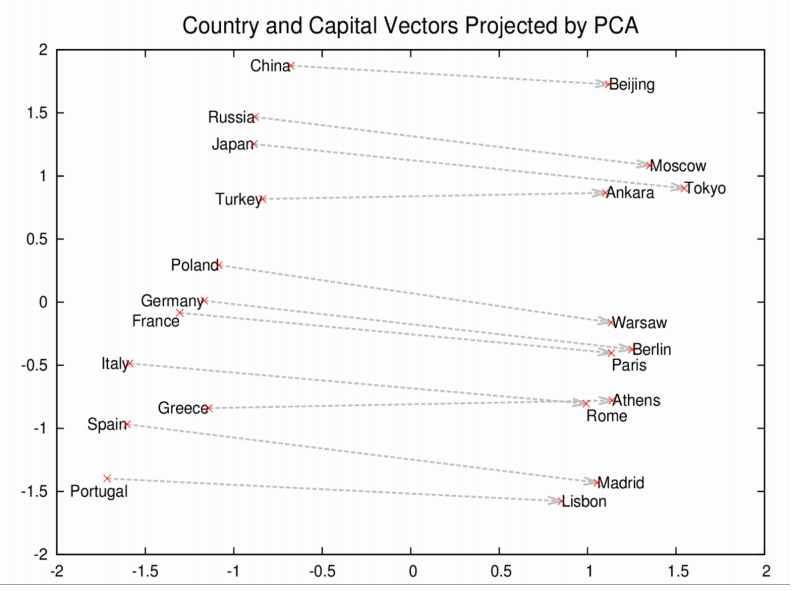
\includegraphics[width=0.44\textwidth]{../images/countries_capitals.png}
		\end{center}
		\pause
		{\scriptsize Japan -- Tokyo $\approx$ Germany -- Berlin }
\end{itemize}
}


\pagestepalt{Applications of Word Vectors}{
\begin{itemize}
	\item \textbf{\href{http://research.microsoft.com/en-us/um/people/cburges/tech_reports/msr-tr-2011-129.pdf}{Sentence Completion}} (actually just restricted language modeling):
	\item ``All red-headed men who are above the age of {\color{darkblue} [ 800 $|$ seven $|$ twenty-one $|$ 1,200 $|$ 60,000 ]} years , are eligible.''
	\item ``That is his {\color{darkblue} [ generous $|$ mother's $|$ successful $|$ favorite $|$ main~]} fault , but on the whole he's a good worker.''
	\pause
	\item \href{http://arxiv.org/pdf/1301.3781.pdf}{Mikolov et al (2013b)} selected the test word that best predicted the context
\end{itemize}
}

\pagestepalt{Kinds of vector spacess}{
  Vector spaces can be divided into two overall categories:\pause
  \begin{itemize}
  \item Count-based
    \begin{itemize}
    \item Corpus counts (however chosen) are either taken ``literally'' or adjusted by an
      information statistic: pointwise mutual information, local mutual information,
      tf/idf, etc. 
    \end{itemize}\pause
  \item Prediction-based 
    \begin{itemize}
    \item Counts are readjusted by applying machine learning techniques to ``compress'' 
      the data (a form of dimensionality reduction\ldots)
    \item Word contexts no longer necessarily human-comprehensible.
    \end{itemize}
  \end{itemize}
}


\placard{Those were fairly fashionable NLP uses of vector spaces, but\ldots}

\pagestepalt{\ldots classification can also be seen as a vector space problem.}{
  Take the contexts seriously -- as ``documents''.\pause
  \begin{itemize}
  \item Another word for the collection of vectors: a ``term-document matrix.''\pause
    \begin{itemize}
    \item ``Document'' can mean even just a few words context, for example.\pause
    \end{itemize}
  \item Instances are contexts/documents, no longer words.\pause
  \item Words (and anything else) are features of the document.\pause
  \item Classification problem: finding a \alert{hyperplane} that divides up the space.
  \end{itemize}
}

\placard{Part 2: maximum entropy (and neural networks}

\pagestepalt{What makes Na\"{i}ve Bayes na\"{i}ve?}{
  \pause
  Na\"{i}ve Bayes assumes that the features are only dependent on the class
  nad independent of one another.\pause
  \begin{block}{Na\"{i}ve Bayes classifier}
      \[\hat{y} = \argmax_y p(y) \prod^n_{i=1} p(x_i | y)\]
  \end{block}
  where $\hat{y}$ is the class chosen by the classifier, $y \in Y$
  where $Y$ is the set of classes, and $x_i$ is the $i$th feature of
  instance $x$.\pause
  \begin{itemize}
  \item Can be estimated directly from the training data. \pause
  \item Look ma, no regression -- computationally relatively cheap. \pause
  \end{itemize}
  But what if the features are \textbf{somewhat} interdependent?\\
  (i.e., most of the time for language\ldots)
}

\pagestepalt{Maximum entropy classifier}{
  ``Maximum entropy classifier'' has a lot of different names for the same
  thing or slightly different related concepts, e.g.:
  \begin{itemize}
  \item Multiclass logistic regression
  \item Softmax regression
  \item Multinomial logit
  \item etc etc etc
  \end{itemize}\pause
  When do you use it? Among other things:\pause
  \begin{itemize}
  \item When you can't guarantee that the data are conditionally independent.\pause
  \item (Like, you know, with language.)\pause
  \item When you still need something that isn't too hard on memory and CPU.
  \end{itemize}
}

\pagestepalt{Maximum entropy classifier}{
  \vspace{-1.0cm}
  Like Na\"{i}ve Bayes, it looks like maximizing a probability:\pause
  \begin{block}{General form of a log-linear model}
      \[P(y|\mathbf{x}) = \text{softmax}(\mathbf{w}_y \cdot \mathbf{x}) = \frac{e^{\mathbf{w}_y \cdot \mathbf{x}}}{Z}\]
  \end{block}\pause
  where $y$ is the class, $\mathbf{w}_y$ is a weight vector
  \alert{specific to that class}, $\mathbf{x}$ is the instance feature
  vector, and $Z$ is the \textbf{normalization constant}.\pause
  \begin{block}{Normalization constant}
    \[Z = \sum_h^Y e^{\mathbf{w}_h \cdot \mathbf{x}}\]
  \end{block}
  where $Y$ is the set of classes.\pause\\
  This can also be called a ``normalized sigmoid function''. 
}

\placard{Which means that we need to learn weights \alert{for every class} that represent the relationships between features and classes.}
      
\pagestepalt{Visualizing the weight matrix}{
  As weight matrices:
  \begin{block}{}
    \begin{center}
      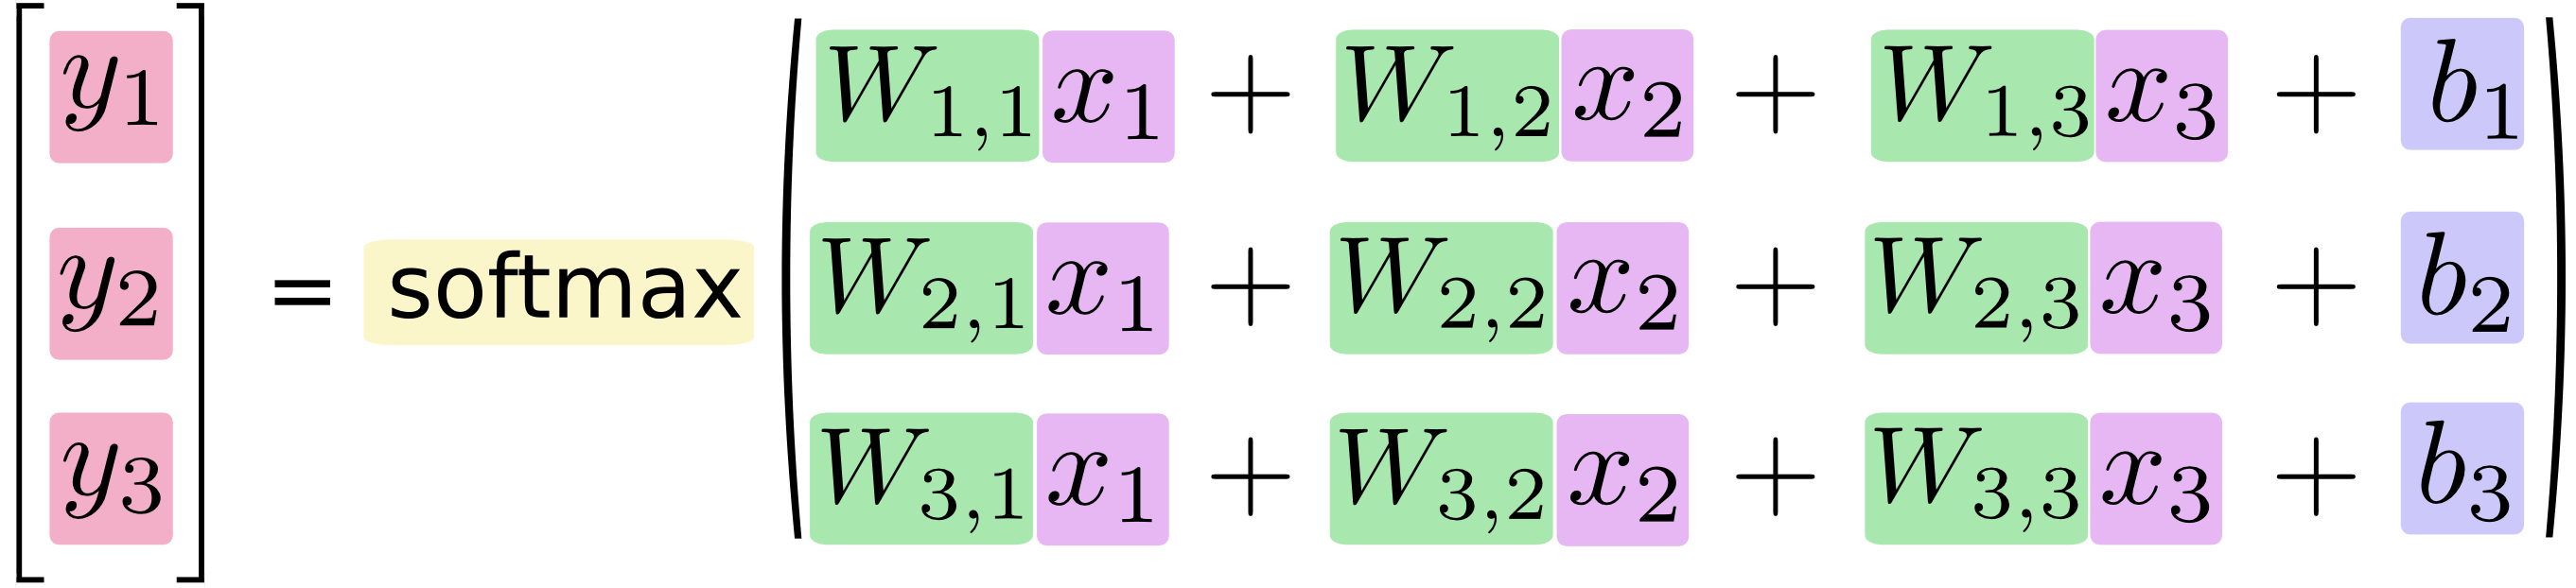
\includegraphics[height=0.19\textheight]{../images/softmax-regression-scalarequation.png} \\[1.1em]\pause
      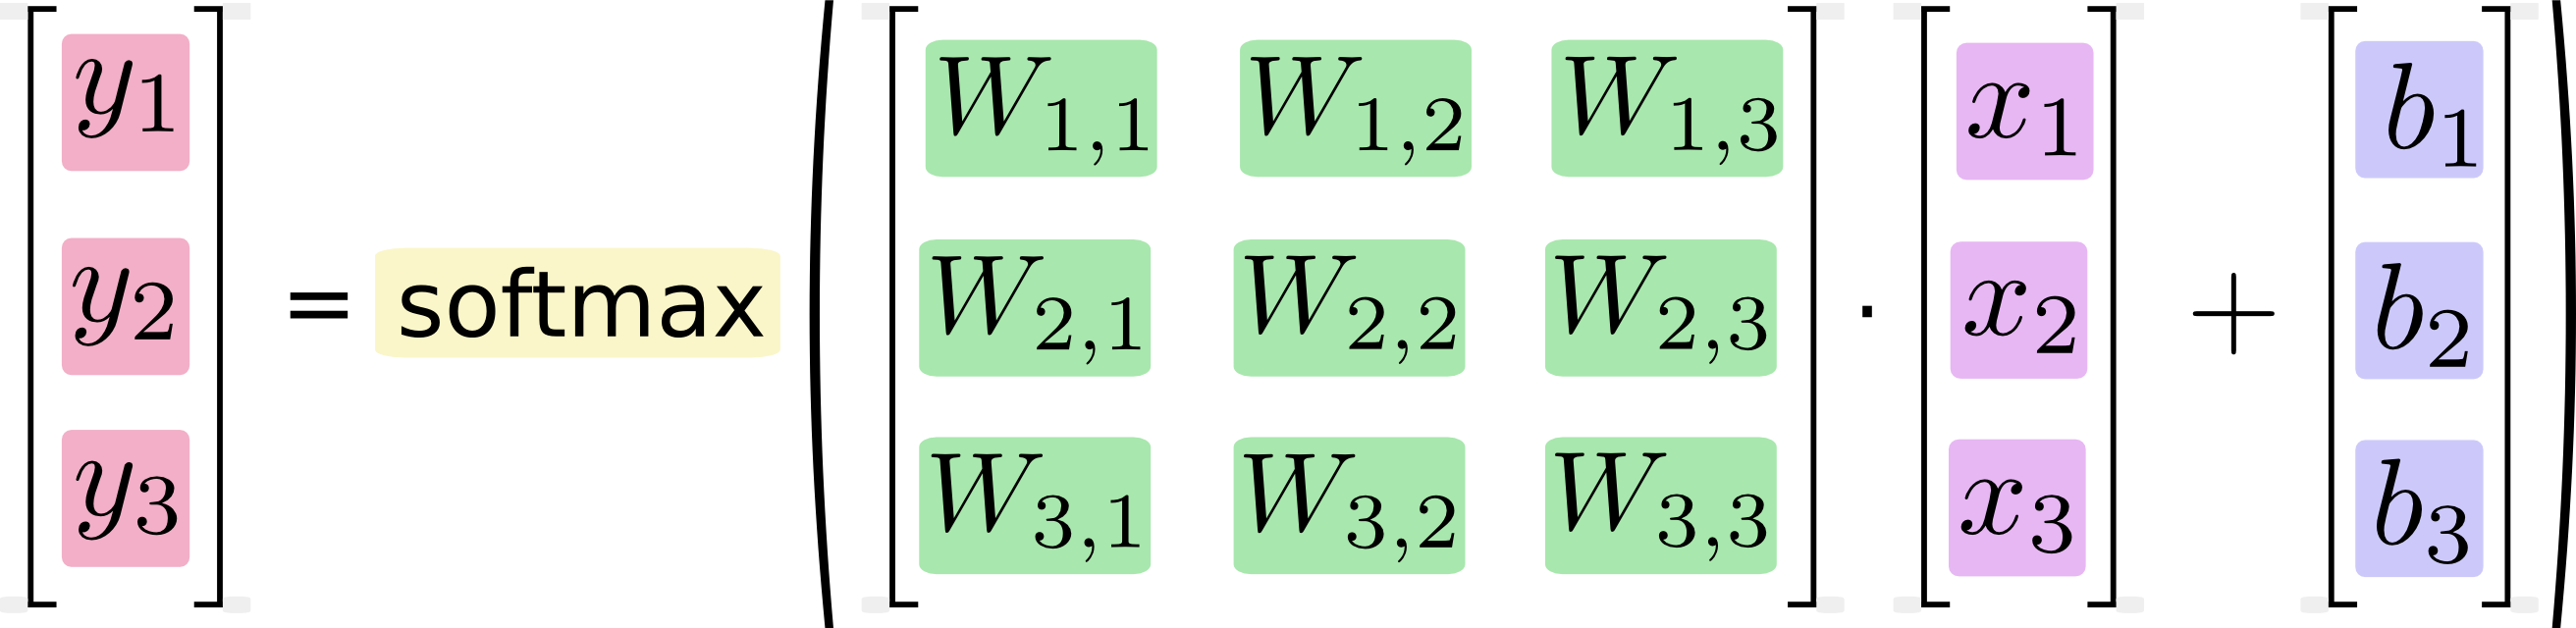
\includegraphics[height=0.19\textheight]{../images/softmax-regression-vectorequation.png} \\[1.1em]
    \end{center}
  \end{block}\pause
  We still need the bias vector $\mathbf{b}$ (remember the intercepts?).\\
  {\tiny Courtesy of \href{http://www.tensorflow.org/tutorials}{TensorFlow}}
}

\pagestepalt{MaxEnt as neural network}{
  \begin{block}{}
    \begin{center}
      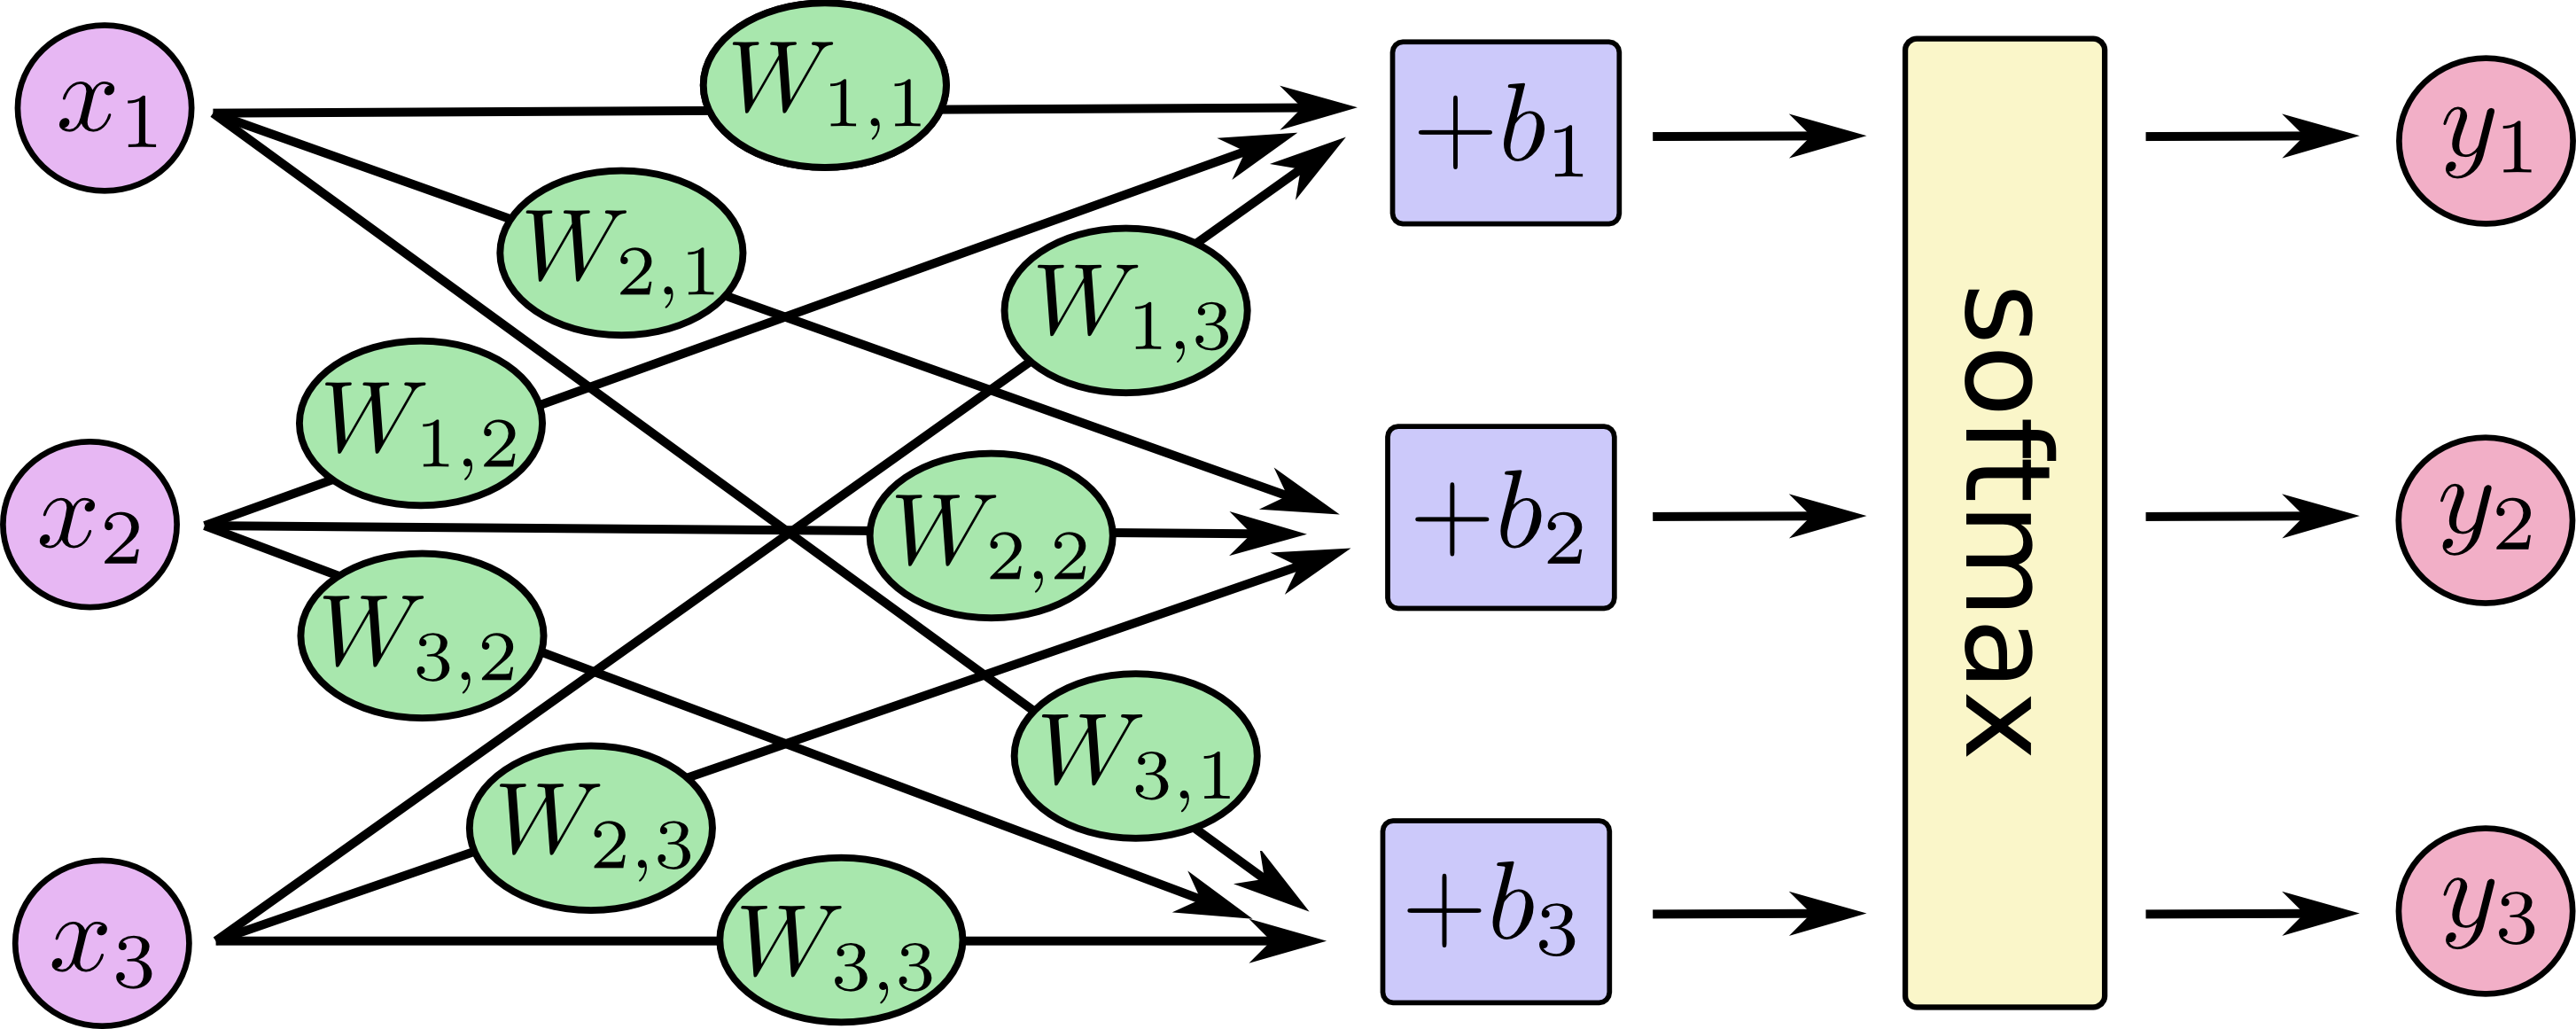
\includegraphics[height=0.29\textheight]{../images/softmax-regression-scalargraph.png}
    \end{center}
  \end{block}\pause
  Another way to think of the bias term is that we set one input
  neuron $x_n$ to $1.0$ permanently.\\\pause
  Finding the weight matrix $\mathbf{W}$ involves numerical optimization
  tricks we won't get into, but one possibility is a form of gradient descent.
  {\tiny Courtesy of
    \href{http://www.tensorflow.org/tutorials}{TensorFlow}}
}

\pagestepalt{Why ``entropy''?}{
  \vspace{-1.5cm}
  Intuition behind maximum entropy classification: expected value of features.
  \vspace{-0.6cm}
  \begin{itemize}
  \item Consider a feature function:
    \begin{block}{}
      \[
      f(\mathbf{x}, y) =
      \begin{cases}
        1 & \text{if class is } y \text{ and } \mathbf{x} \text{ has given feature}  \\
        0 & \text{otherwise}
      \end{cases}
      \]
    \end{block}\pause
  \item Then we can compute the expected value of the feature from the empirical feature distribution $\tilde{p}(x)$.
    \begin{block}{}
      \[p(f) = \sum_{x,y} \tilde{p}(x)p(y|x)f(x,y)\]
    \end{block}\pause
  \item Problem is, we don't know the model $p(y|x)f(x,y)$, so we
    instead maximize its entropy $-\sum p(y|x) \log p(y|x)$.\pause
  \item The optimization problem can be parameterized via $e$ and weights.
  \end{itemize}
}

\placard{\ldots but back to dimensionality reduction!}

\placard{Part 3: Beyond LSA}

\pagestepalt{Autoencoder}{
  \vspace{-0.6cm}
  From Stanford deep learning tutorial:
  \begin{center}
    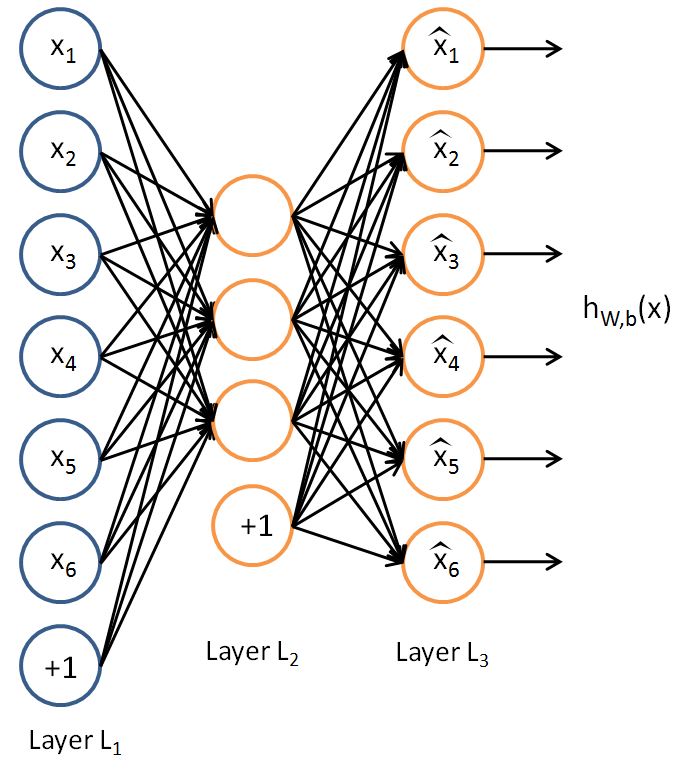
\includegraphics[width=0.4\textwidth]{autoencoder.png}
  \end{center}
  Learn compressed representation of the input by learning the
  identity function via a neural network.
}


% models, relationship with projection layers of nnlm's
\pagestepalt{Projection Layer in Neural Language Models}{
\begin{itemize}
	\item \textbf{Neural Language Modeling} -- this was actually one of the earliest uses of word vectors.  We'll talk more about these next semester \\
		\begin{center}
		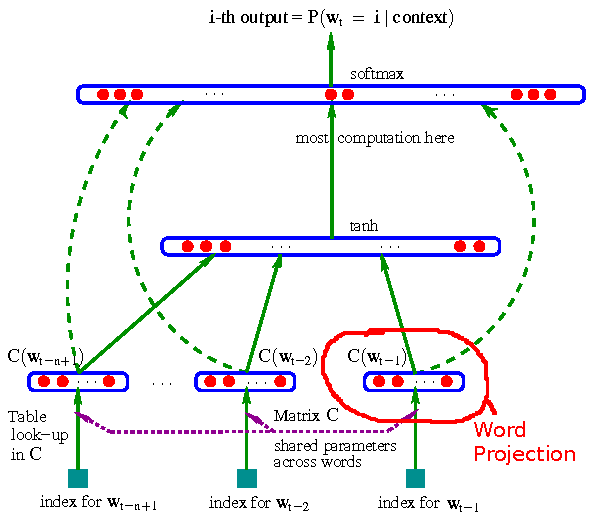
\includegraphics[width=0.55\textwidth]{../images/bengio-etal2003_pg6_image_alt.pdf}
		\end{center}
\end{itemize}
}


% word2vec: cbow, sg
\pagestepalt{word2vec}{
\begin{itemize}
	\item Tom\'{a}\v{s} Mikolov and colleagues found that you don't need the full neural-net language model to get useful word vectors
	\pause
	\item In fact, you don't need a neural network at all. He removed the hidden layer, giving a traditional log-linear model
	\pause
	\item He developed a simplified form of training called negative sampling (derived from earlier NCE).  It's a little like a binary MaxEnt classifier
\end{itemize}
}


\pagestepalt{word2vec: CBOW \& Skip-gram}{
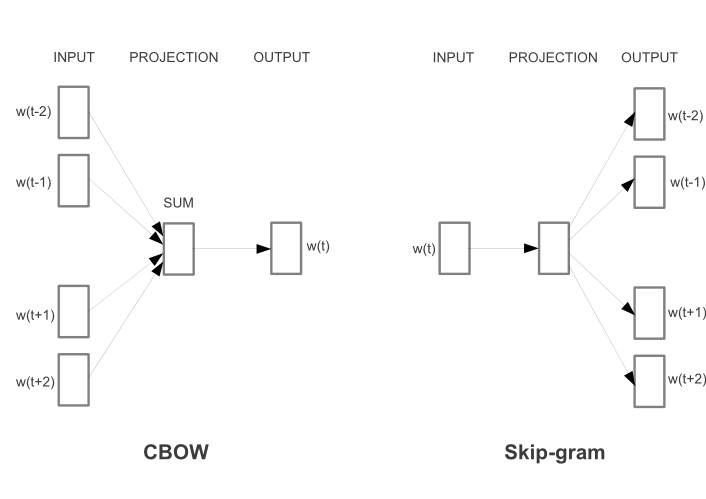
\includegraphics[width=0.90\textwidth]{../images/mikolov-etal2013b_fig1.png}
%\begin{itemize}
%	\item 
%	\item 
%\end{itemize}
}


\pagestepalt{Hyperparameters}{
  (What is a parameter? Usually, the model weights. Example hyperparameter: how many parameters\ldots)\pause
\begin{itemize}
	\item Window size: how much surrounding context to use
	\item Normalization: softmax (traditional) vs.\ hierarchical softmax vs.\ negative sampling
	\item Vector dimensions: 100--500 common
	\item Number of negative samples: 3--10 common
	\item Number of training epochs, initial learning rate, negative sample distribution ($\alpha = 0.75$), model, \ldots
\end{itemize}
}

\placard{Assignment 1 is due next week and assignment 2 will come out too\ldots}

\end{document}
